
Here is \cref{sec1:res:tab:time_of_events}

\begin{table}[ht!]
    \centering
    \begin{tabular}{|l|c|c|c|}
        \hline
        \textbf{Event} & \multicolumn{3}{c|}{\textbf{Time}} \\
        \hline
        % \textbf{Event} & \textbf{Conformal time} $x$ & \textbf{Redshift} $z$ & \textbf{Cosmic time} $t$ \\
         & $x$ & $z$ &  $t$ \\
        \hline
        R-M equality & $-8.67$ &  & \\
        M-DE equality & &  & \\
        $\ddot{a}>0$ & &  & \\
        today  & &  & $13.86$ Gyrs \\
        $\eta(0)/c$ & &  & \\
        \hline
    \end{tabular}
    \caption{The logarithmic scale factor ($x$), redshift ($z$) and cosmic time ($t$) of various milestones in the history of the universe.}
    \label[tab]{sec1:res:tab:time_of_events}
\end{table}



This is \cref{sec1:res:fig:hubble} from \citep{2006astro.ph..6683C}



\begin{figure}[!ht]
    \centering
    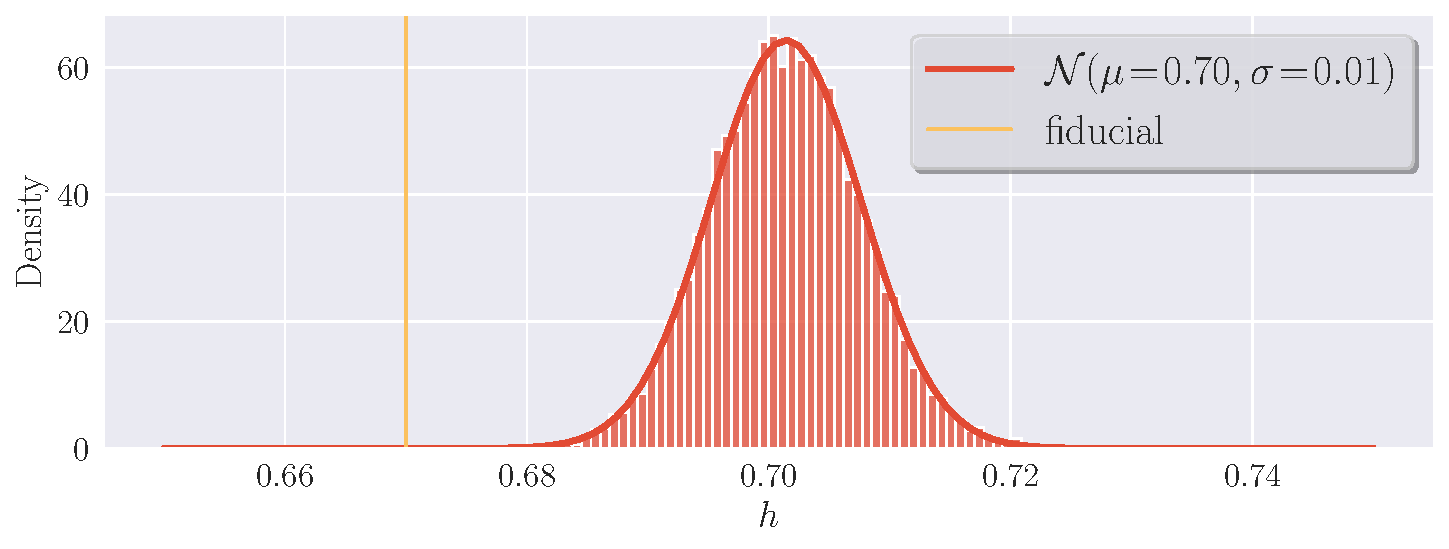
\includegraphics[width=\linewidth]{milestone1/hubble_pdf.pdf} 
    \caption{Duration as} 
    \label[fig]{sec1:res:fig:hubble}
\end{figure} 